\documentclass[jrfm,article,submit,moreauthors,pdftex]{Definitions/mdpi}

\usepackage{tabularx}
\setlength{\headheight}{20pt}

\firstpage{1}
\pubyear{2026}
\copyrightyear{2026}
\doinum{}
\datereceived{}
\daterevised{}
\dateaccepted{}
\datepublished{}

\Title{Does Volatility Persistence Forecast Volatility? Rolling Long Memory, Crisis Windows, and Implied Volatility}


% CO-AUTHORS TO CONFIRM: author order, Hongwei Mei's affiliation, corresponding author.
\Author{Akash Deep $^{1}$, Nicholas Appiah $^{1,*}$, Hongwei Mei $^{1}$ and Svetlozar T. Rachev $^{1}$}
\AuthorNames{Akash Deep, Nicholas Appiah, Hongwei Mei and Svetlozar T. Rachev}

\address[1]{Department of Mathematics and Statistics, Texas Tech University,
Lubbock, TX 79409, USA}
\corres{Correspondence: \href{mailto:niappiah@ttu.edu}{niappiah@ttu.edu}}

\abstract{Rolling estimates of long memory in volatility rise sharply in
crises and are often read as a time-varying state of the market. We ask
whether this state forecasts stock volatility beyond implied volatility, and
what it measures. For 115 S\&P~500 stocks over 2001--2026 we forecast log
Parkinson variance one day, one week and one month ahead with per-stock HAR
models, with HAR plus the VIX and MOVE indices (HAR-X), and with
specifications that add own-stock, sector and cross-sectional persistence.
All forecasts are point-in-time, the designs were fixed before their results
were computed, and inference combines panel Diebold--Mariano, Clark--West and
Giacomini--White tests. Persistence never improves on HAR-X: the best gain is
0.26\% at one week and is not significant, and the full model is
significantly worse at one day and one month. Pooled estimation, a
term-structure target, a market-level series and five machine-learning
estimators agree. The reason is mechanical. The persistence state jumps when
an extreme episode enters the estimation window and falls when it leaves,
at dates that move one-for-one with the window length; a short-memory model
reproduces the pattern; and the largest VIX inside the window explains 83\%
of its variation. A one-day misalignment between HAR inputs and the VIX
inflates the VIX's apparent forecasting gain by about a third.}

\keyword{long memory; volatility forecasting; implied volatility; HAR model;
rolling-window estimation; spurious long memory; forecast evaluation}

\begin{document}

\section{Introduction}\label{sec:intro}

Volatility is persistent. Shocks to the variance of stock returns decay
slowly, the autocorrelations of squared and absolute returns stay positive
for months, and the log-periodogram of realized variance rises steeply
toward the origin \citep{ding1993long, andersen2003modeling}. A large
literature models this with fractional integration of order $d$, and an
equally large applied literature estimates $d$, or the related Hurst
exponent, over rolling windows and reads the resulting series as a
time-varying property of the market: persistence that strengthens in
crises, efficiency that improves or deteriorates, or adaptive behaviour in
the sense of \citet{lo2004adaptive}. Examples range from early work on
the Hurst exponent over time \citep{cajueiro2004hurst} to recent studies of
volatility persistence after COVID-19 \citep{veravaldes2022persistence} and
of the pandemic's effect on market efficiency \citep{takaishi2025}.

If rolling persistence is a genuine state of the market, it should carry
information about future volatility. This paper tests that implication and,
when it fails, asks why. We pose two questions. First, does a persistence
state built from rolling long-memory estimates forecast stock volatility
beyond what implied volatility already contains? Second, what does the
rolling persistence state measure?

We answer both on a panel of 115 S\&P~500 stocks from November 2001 to April
2026. Volatility is the daily Parkinson range variance, and the forecast
target is the log of its mean over the next 1, 5 or 22 trading days. The
benchmarks are the heterogeneous autoregressive (HAR) model of
\citet{corsi2009simple} and a HAR model augmented with the closing levels of
the VIX and MOVE indices (HAR-X). The persistence state enters through
own-stock rolling estimates of $d$, sector and cross-sectional averages of
those estimates, and their interactions with implied volatility. Every
forecast is point-in-time: predictors use information available at the close
of the forecast origin, and a training row enters a regression only if its
target window has closed by the origin. Each specification and its decision
rule were recorded in a dated experiment ledger before its results were
computed. Inference combines the panel Diebold--Mariano test with the
\citet{harvey1997testing} correction, the \citet{clark2007approximately} test
for nested models and the conditional predictive ability test of
\citet{giacomini2006tests}.

The answer to the first question is no. Implied volatility improves on HAR
by 3.1\%, 5.5\% and 1.8\% in mean squared error at the three horizons.
Persistence adds nothing on top. The best gain over HAR-X is 0.26\% at one
week, with a Diebold--Mariano statistic of 0.41, and the full model is
significantly worse than HAR-X at one day and one month. Pooled estimation
with stock fixed effects, a target that measures the slope of the variance
term structure, a single market-level series, and five machine-learning
estimators all give the same answer. The Clark--West test rejects the null
that the persistence terms have zero population coefficients, but the
Giacomini--White test never finds that the estimated models forecast better:
the information exists in population and cannot be extracted in practice.

The answer to the second question explains the first. The cross-sectional
mean of rolling $d$ estimates behaves as an indicator of whether a large,
long volatility episode lies inside the estimation window. It jumps when
such an episode enters the window and falls when the episode leaves, and the
exit date moves one-for-one with the window length: for windows of 500, 750
and 1{,}000 trading days the 2020 plateau ends on 11 March 2022, 10 March
2023 and 8 March 2024, each time with a fall in the bottom 0.2\% of all
weekly changes. A short-memory ARMA model fitted to calm-period data, with the
observed 2020 episode added, reproduces the calm level of the estimate, the
plateau and the exit. The largest VIX inside the window explains 81--83\% of
the variation in the state, against 18--28\% for the current VIX. A state
that is a lagged summary of past extreme episodes has little to add to an
implied-volatility index that already prices them.

A third result is practical. If HAR inputs end one day before the forecast
origin while the VIX is the origin-day close, HAR is handicapped and the
VIX's gain is overstated by about a third. With aligned inputs HAR's error
falls by 8.1\% at the daily horizon and the VIX's gain over HAR falls from
5.1\% to 3.1\%.

These results connect to three literatures. The first shows that structural
breaks, level shifts and regime switching produce spurious evidence of long
memory \citep{diebold2001long, granger2004occasional,
mikosch2004nonstationarities, smith2005level, perron2010long}, with tests and
estimators designed to tell the two apart \citep{qu2011test,
hou2014modified} and evidence that little genuine long memory survives once
level shifts are modelled \citep{varneskov2018combining}. That literature
concerns full-sample estimates. We document its time-series consequence for
rolling estimates, which are what applied work interprets, and give a simple
check: vary the window and see whether the turning points move with it. The
problem is old in other sciences. Mean shifts were shown to mimic the Hurst
phenomenon in river flows \citep{klemes1974hurst}, the separation of extreme
events from persistence goes back to the ``Noah'' and ``Joseph'' effects of
\citet{mandelbrot1968noah}, patchy composition mimics long-range correlation
in DNA \citep{karlin1993patchiness}, and rolling-window indicators of
critical slowing down and of dynamic brain connectivity have faced the same
critique \citep{dakos2008slowing, ditlevsen2010tipping,
boettiger2012quantifying, leonardi2015spurious}.

The second literature compares implied and time-series forecasts of
volatility \citep{christensen1998relation, fleming1998quality,
blair2001forecasting, busch2011role} and documents a variance risk premium
that varies with conditions \citep{bates2000post, chernov2007role,
bekaert2014vix, andersen2015risk}. Our timing result adds a concrete pitfall
to that comparison. The third literature asks whether volatility is rough
\citep{gatheral2018volatility, fukasawa2022consistent, cont2024rough} and
whether volatility forecasts create value in managed portfolios
\citep{moreira2017volatility, cederburg2020volatility,
barroso2021volatility}. We report both briefly: a roughness estimate of 0.06
on daily range data is reproduced by a non-rough model with measurement
noise, and managed portfolios built on any of our forecasts have the same
Sharpe ratio as the equal-weighted portfolio once returns are measured in
excess of the bill rate.

The paper proceeds as follows. Section~\ref{sec:data} describes the data
and the full-sample memory estimates. Section~\ref{sec:window} shows what
the rolling persistence state measures. Section~\ref{sec:design} sets out
the forecasting design and Section~\ref{sec:results} the results.
Section~\ref{sec:robust} reports robustness checks and the portfolio
exercise, and Section~\ref{sec:discussion} discusses implications and
limitations. The appendices collect supplementary results and the
registration record.

\section{Data and Measurement}\label{sec:data}

\subsection{Sample}

Daily open, high, low and close prices for S\&P~500 constituents were
obtained from Bloomberg. The panel keeps the 115 stocks with at least 70\%
of trading days observed between 29 November 2001 and 21 April 2026, a total
of 6136 trading days, and covers all eleven GICS sectors. Membership is that
of the April 2026 index, so the panel excludes firms that left the index
before then; Section~\ref{sec:discussion} discusses what this implies.
Returns are daily log price returns. They are winsorized point-in-time at the
expanding 0.1\% and 99.9\% quantiles after a 500-day warm-up, so that no
observation is trimmed using later data, and one special dividend that
appears as a price drop (Keurig Dr Pepper, 10 July 2018) is added back. The
market variables are the closing levels of the CBOE VIX index and the ICE
BofA MOVE index of Treasury implied volatility, and the three-month Treasury
bill rate.

\subsection{Variance}

Daily variance is measured by the range estimator of
\citet{parkinson1980extreme},
\begin{equation}
\sigma^2_{i,t} = \frac{\left(\ln H_{i,t} - \ln L_{i,t}\right)^2}{4\ln 2},
\label{eq:parkinson}
\end{equation}
where $H_{i,t}$ and $L_{i,t}$ are the day's high and low. The estimator uses
intraday information, is several times more efficient than the squared
close-to-close return, and is available for the full sample, which
five-minute realized variance is not. Days with a zero range are treated as
missing. All models work with the log of variance, which is close to
Gaussian and makes forecast errors comparable across stocks.

\subsection{Timing}

The forecast origin is the close of trading day $t$. Every predictor uses
information available at that moment: the day's range and return, and the
closing levels of the VIX and MOVE indices. The VIX is computed until 4:15
p.m.\ Eastern time, fifteen minutes after the equity close; we treat the two
as simultaneous. The forecast target for horizon $h$ is
\begin{equation}
y_{i,t,h} = \ln\Bigl(\frac{1}{h}\sum_{k=1}^{h} \sigma^2_{i,t+k}\Bigr),
\qquad h \in \{1, 5, 22\},
\label{eq:target}
\end{equation}
the log of mean variance over the next day, week and month. Forecasts are
made every fifth trading day, which gives 1078 weekly origins from 22
November 2004, the first date at which a 750-day window is available, to 21
April 2026. Section~\ref{sec:results} shows that this alignment matters.

\subsection{Full-sample memory}

Table~\ref{tab:memory} reports full-sample estimates of the fractional
parameter $d$ by the log-periodogram estimator of
\citet{geweke1983estimation} (GPH) and the local Whittle estimator of
\citet{robinson1995gaussian}, both with bandwidth $m=T^{0.65}$. Returns show
no memory: the mean estimate is $-0.02$. Log variance shows a great deal: the
mean GPH estimate is 0.54, the local Whittle estimate 0.52, and 84\% of stocks
have a GPH estimate above 0.5, the boundary of stationarity. These are the
familiar stylized facts \citep{andersen2003modeling}. A Hurst exponent of
0.06 from the scaling of increments of log variance would, read literally,
indicate very rough volatility \citep{gatheral2018volatility}; Appendix~\ref{app:rough}
shows that a two-factor Markovian model without roughness, observed through
the sampling noise of the range estimator, produces the same number, so
roughness is not identified at the daily frequency \citep{cont2024rough}. We do not use roughness further.

\begin{table}[H]
\caption{Full-sample memory estimates across the 115 stocks.}
\label{tab:memory}
\small
\begin{tabularx}{\textwidth}{Xcccccc}
\toprule
Series & Estimator & Mean & 10th pct & Median & 90th pct & Share $>0.5$ \\
\midrule
Returns & GPH & -0.020 & -0.082 & -0.022 & 0.044 & 0\% \\
 & LW & -0.027 & -0.077 & -0.027 & 0.025 & 0\% \\
Log Parkinson variance & GPH & 0.538 & 0.490 & 0.537 & 0.587 & 84\% \\
 & LW & 0.516 & 0.476 & 0.515 & 0.559 & 70\% \\
Log Parkinson variance & Hurst ($q=2$) & 0.060 & 0.053 & 0.060 & 0.069 & -- \\
\bottomrule
\end{tabularx}
\noindent{\footnotesize{\textit{Notes:} Daily data, 29 November 2001 to 21 April 2026 (6136 trading days). GPH: log-periodogram estimator of the fractional parameter $d$; LW: local Whittle; bandwidth $m=T^{0.65}$. Hurst: scaling of second moments of increments of log variance over lags 1 to 21 days. Percentiles are across stocks.}}
\end{table}


Estimates of $d$ above 0.5 for most stocks are themselves a warning. Long
memory and a slowly decaying short-memory process with occasional large
episodes are hard to tell apart in samples of this length
\citep{diebold2001long, granger2004occasional}. The rolling estimates that
follow make the distinction visible.

\section{What the Rolling Persistence State Measures}\label{sec:window}

\subsection{The state}

For each stock and weekly origin, $\hat d_{i,t}(W)$ denotes the GPH estimate
computed from the $W$ log-variance observations ending on day $t$, with
$W=750$ in the baseline. The persistence state is the cross-sectional mean
$\bar d_t(W) = N^{-1}\sum_i \hat d_{i,t}(W)$, together with its
cross-sectional standard deviation. The state rises sharply in crises: it
averages about 0.38 in calm years and 0.57 while the 2020 episode is inside
the window. Read as a property of the market, this would mean that shocks to
volatility became markedly more persistent after March 2020 and remained so
for three years.

\subsection{A mechanical account}

A simpler account predicts the same rise and makes three further predictions
that the persistence interpretation does not. Suppose that log variance is a
short-memory process plus a temporary episode, a block of elevated values of
height $b$ and length $L$. Within a window of length $W$, the episode adds a
component to the discrete Fourier transform whose modulus at the Fourier
frequency $\lambda_j = 2\pi j/W$ is
$b\,\lvert\sin(L\lambda_j/2)/\sin(\lambda_j/2)\rvert$. This modulus is large
at frequencies below about $2\pi/L$ and does not depend on the position of
the episode within the window, because shifting the episode changes only the
phase. The log-periodogram estimator regresses the log periodogram on log
frequency over the lowest $m$ frequencies, so the additional low-frequency
power raises $\hat d$. Three predictions follow. First, the estimate jumps
when the episode enters the window, stays roughly constant while the episode
is inside, and falls when it leaves; the fall therefore occurs $W$ days after
the episode and moves one-for-one with the window length. Second, the size
of the effect increases with the duration of the episode, not only with its
peak, so a one-day crash should have little effect. Third, the state should
track the largest recent episode more closely than the current level of
volatility. None of these predictions requires the persistence of shocks to
change.

\subsection{Evidence}

The events are fixed in advance as the three largest days of cross-sectional
mean log variance that lie at least 250 trading days apart: 10 October 2008,
6 May 2010 (the Flash Crash) and 18 March 2020. For each event and window
length $W\in\{500, 750, 1000\}$, Panel A of Table~\ref{tab:window} compares
the mean state over the four weeks after the event day enters the window
with the mean over the four weeks before, and does the same when the day
leaves the window $W$ trading days later. Each change is ranked among all
four-week changes in the series.

\begin{table}[H]
\caption{What the rolling persistence state tracks.}
\label{tab:window}
\footnotesize
\begin{tabularx}{\textwidth}{lXXXXXX}
\toprule
\multicolumn{7}{l}{\textit{Panel A. Change in $\bar d_t(W)$ when the event day enters and leaves the window (percentile among all changes)}} \\
\midrule
Event & $W$ & Entry & Pct & Exit date & Exit & Pct \\
\midrule
2008-10-10 & 500 & +0.159 & 99.8 & 2010-10-06 & +0.009 & 80.8 \\
 & 750 & +0.093 & 99.6 & 2011-10-03 & -0.065 & 0.8 \\
 & 1000 & +0.104 & 99.5 & 2012-09-28 & -0.036 & 1.7 \\
2010-05-06 & 500 & -0.008 & 22.7 & 2012-04-30 & -0.000 & 51.6 \\
 & 750 & +0.012 & 90.4 & 2013-04-30 & -0.017 & 9.6 \\
 & 1000 & +0.002 & 65.9 & 2014-04-28 & -0.022 & 5.4 \\
2020-03-18 & 500 & +0.181 & 99.9 & 2022-03-11 & -0.164 & 0.2 \\
 & 750 & +0.125 & 99.9 & 2023-03-10 & -0.108 & 0.1 \\
 & 1000 & +0.108 & 99.7 & 2024-03-08 & -0.090 & 0.1 \\
\midrule
\multicolumn{7}{l}{\textit{Panel B. $R^2$ of $\bar d_t(W)$ on the VIX}} \\
\midrule
& $W$ & \multicolumn{2}{c}{Max VIX in window} & & \multicolumn{2}{c}{Current VIX} \\
\midrule
& 500 & \multicolumn{2}{c}{0.81} & & \multicolumn{2}{c}{0.28} \\
& 750 & \multicolumn{2}{c}{0.83} & & \multicolumn{2}{c}{0.27} \\
& 1000 & \multicolumn{2}{c}{0.82} & & \multicolumn{2}{c}{0.18} \\
\midrule
\multicolumn{7}{l}{\textit{Panel C. The 2020 episode: data versus a short-memory null}} \\
\midrule
& $W$ & Before & Inside & After exit & Rise & Largest drop \\
\midrule
Data & 500 & 0.35 & 0.60 & 0.33 & +0.25 & \\
Null & 500 & 0.41 & 0.54 & 0.47 & +0.13 & day 509 \\
Data & 750 & 0.38 & 0.57 & 0.33 & +0.19 & \\
Null & 750 & 0.40 & 0.53 & 0.46 & +0.13 & day 759 \\
Data & 1000 & 0.37 & 0.53 & 0.34 & +0.16 & \\
Null & 1000 & 0.39 & 0.50 & 0.44 & +0.11 & day 1009 \\
\bottomrule
\end{tabularx}
\noindent{\footnotesize{\textit{Notes:} $\bar d_t(W)$ is the cross-sectional mean of the GPH estimate on log Parkinson variance over the $W$ trading days ending on day $t$, on the weekly grid. Events are the three largest days of cross-sectional mean log variance at least 250 days apart (rule fixed in advance). Entry and exit changes compare the four weekly estimates after the date with the four before; Pct is the percentile of that change among all such changes. Panel C: mean $\bar d_t$ in the 120 days before the event, from day 60 to day $W-60$, and from day $W+20$ to $W+120$. The null is an ARMA(1,1) with the median parameters of per-stock fits to 2012--2019 log variance plus the observed one-year 2020 excess log variance, 200 replications; Largest drop is the day (relative to the event) of its largest four-week fall.}}
\end{table}


The 2020 event produces the predicted pattern at every window length. The
state rises by 0.11 to 0.18 on entry, among the largest 0.3\% of changes, and
falls by 0.09 to 0.16 on exit, among the smallest 0.2\%. The exit dates are
11 March 2022, 10 March 2023 and 8 March 2024. Figure~\ref{fig:window} shows
the three series: each holds a plateau and drops on its own exit date. The
October 2008 event shows the same pattern at 750 and 1000 days. At 500 days
its exit is masked because the remainder of the 2008--2009 episode and the
May 2010 turmoil are still inside the window. The Flash Crash, a single
extreme day, barely moves the state on entry or exit, as the second
prediction requires.

Panel B tests the third prediction. The largest VIX close inside the same
window explains 81--83\% of the variation in the state at every window
length, whereas the current VIX explains 18--28\%. Most of the variation in
the state is therefore accounted for by a single observable, the highest VIX
close in the estimation window.

\begin{figure}[H]
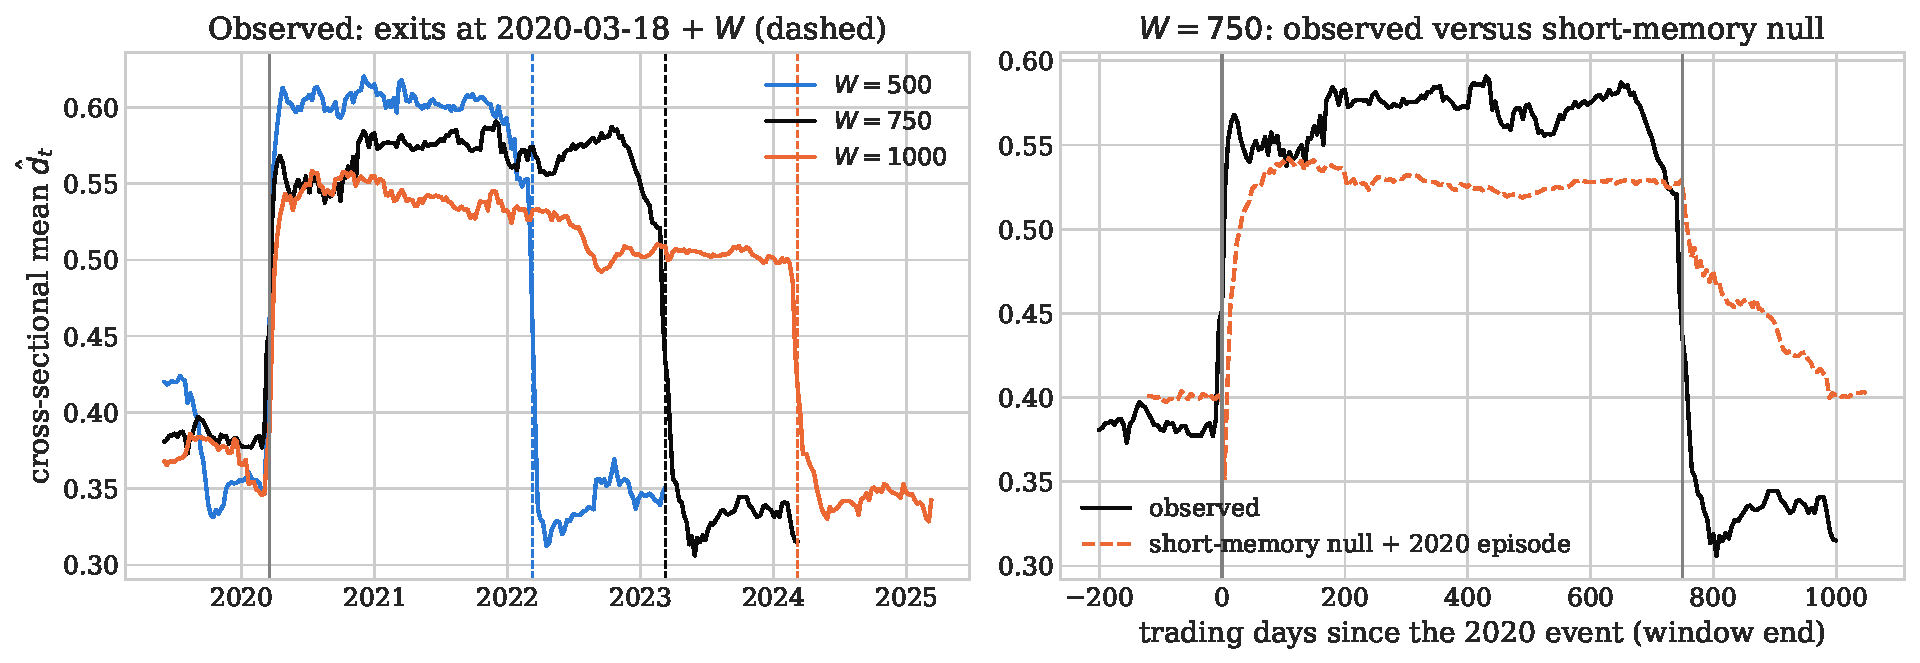
\includegraphics[width=\textwidth]{figures/fig10_window_inclusion.pdf}
\caption{The persistence state around the 2020 episode. Left: cross-sectional
mean of the rolling GPH estimate for windows of 500, 750 and 1000 trading
days; the solid gray line marks 18 March 2020 and the dashed lines the dates
on which that day leaves each window. Right: the 750-day series in event
time and the mean of 200 simulations of a short-memory ARMA(1,1) process,
fitted to 2012--2019 data, with the observed 2020 excess log variance
added.}
\label{fig:window}
\end{figure}

Panel C and the right panel of Figure~\ref{fig:window} ask whether a process
without long memory can generate this pattern. We fit an ARMA(1,1) model to
each stock's log variance over 2012--2019, a period without an episode of
the scale of 2008 or 2020, take the median parameters ($\phi=0.91$,
$\theta=-0.69$), add the observed cross-sectional median excess log variance
of the year after 18 March 2020, and apply the same rolling estimator to 200
simulated paths. The simulated state starts at 0.40, close to the observed
0.385, rises on entry, holds a plateau, and has its largest fall within nine
days of the exit date at every window length. It reproduces 53--69\% of the
observed rise. A shortfall is to be expected, since the null contains a
single stylized episode with the cross-sectional median profile, whereas each
stock's window in the data also contains its own later shocks of 2020--2022.

\subsection{Implications}

Two implications matter for what follows. First, a persistence state built
from rolling long-memory estimates is a lagged and smoothed record of how
much extreme volatility has occurred over the past few years. Implied
volatility already reflects that history, partly through the variance risk
premium, which rises after crises and decays slowly \citep{bates2000post,
andersen2015risk}. There is therefore little reason to expect the state to
add forecasting information, and Sections~\ref{sec:results} and
\ref{sec:robust} find that it does not.

Second, rolling memory estimates should not be read as evidence of changing
persistence or efficiency without checking how their turning points depend on
the window. The dates illustrate the risk. With a 750-day window the 2020
shock leaves the window on 10 March 2023, the day Silicon Valley Bank
failed; with a 500-day window it leaves on 11 March 2022, two weeks after
Russia invaded Ukraine. A study based on a single window could plausibly
attribute the fall in persistence to one of those events. Varying the window
and checking whether the turning points move with it is an inexpensive
safeguard. Our evidence concerns memory in volatility; whether rolling
estimates of memory in returns behave in the same way depends on the
estimator and is left for future work.

\section{Forecasting Design}\label{sec:design}

\subsection{Models}

All models are linear regressions of the target \eqref{eq:target} on
predictors dated $t$, estimated stock by stock. The baseline, model $A$, is
the HAR model of \citet{corsi2009simple} in logs with a return term,
\begin{equation}
y_{i,t,h} = \beta_0 + \beta_d \ln RV^{(1)}_{i,t} + \beta_w \ln RV^{(5)}_{i,t}
+ \beta_m \ln RV^{(22)}_{i,t} + \gamma_1 r_{i,t} + \gamma_2 \lvert r_{i,t}\rvert
+ \varepsilon_{i,t,h},
\label{eq:har}
\end{equation}
where $RV^{(k)}_{i,t}$ is the mean Parkinson variance over days $t-k+1$ to
$t$, and $r_{i,t}$ is the return on day $t$. HAR-X, model $A_1$, adds the
levels of the VIX and MOVE indices at the close of day $t$. The persistence
blocks are added to HAR one at a time and then jointly. Three further
specifications, fixed before their results were computed, add a single block
to HAR-X, so that the comparison with HAR-X isolates that block.
Table~\ref{tab:models} lists the predictors.

\begin{table}[H]
\caption{Model specifications.}
\label{tab:models}
\footnotesize
\begin{tabularx}{\textwidth}{lX}
\toprule
Model & Predictors \\
\midrule
$A$ (HAR) & $\ln RV^{(1)}, \ln RV^{(5)}, \ln RV^{(22)}, r_t, \lvert r_t\rvert$ \\
$A_1$ (HAR-X) & HAR + VIX, MOVE \\
$A_2$ & HAR + own-stock $\hat d_{i,t}$, its weekly change, its standard deviation and slope over four weeks, own Hurst exponent and its weekly change \\
$A_3$ & HAR + cross-sectional mean $\bar d_t$ and dispersion $\sigma_{d,t}$ \\
$A_4$ & HAR + leave-one-out sector mean of $\hat d_{i,t}$ \\
$A_5$ & HAR + $\hat d_{i,t}$, VIX, MOVE, $\hat d_{i,t}\times$VIX, $\hat d_{i,t}\times$MOVE \\
$C$ & Union of $A_1$ to $A_5$ (18 predictors) \\
\midrule
\multicolumn{2}{l}{\textit{Registered HAR-X extensions}} \\
HAR-X + cross-sectional state & HAR-X + $\bar d_t$, $\sigma_{d,t}$ \\
HAR-X + sector state & HAR-X + leave-one-out sector mean of $\hat d_{i,t}$ \\
HAR-X + state $\times$ HAR terms & HAR-X + $\bar d_t$ and $\bar d_t\times \ln RV^{(k)}_{i,t}$, $k=1,5,22$ \\
\bottomrule
\end{tabularx}
\noindent{\footnotesize{\textit{Notes:} All predictors are dated at the close
of the origin day $t$. Rolling estimates use the 750 trading days ending on
day $t$. The last specification lets the persistence state change the
weights on the HAR components, the channel through which slower decay of
shocks would act.}}
\end{table}

\subsection{Estimation}

Each model is re-estimated by ordinary least squares at every weekly origin
on an expanding window of that stock's past observations. Because targets
overlap for $h>1$, a past observation enters the regression only if its
target window has closed by the origin: the observation for an earlier
origin $s$ is used at origin $t$ only if its target window, days $s+1$ to
$s+h$, ends no later than day $t$. Without this restriction the last
observations of each training sample contain variance that has not yet been
realized; at $h=22$ this inflated the apparent gain of the richer models in
an earlier version of this study. The first 431 origins (up to 14 June 2013)
form the initial training sample, and all models are evaluated over the same
646 origins, from 17 June 2013 to 14 April 2026, on the same (date, stock)
cells.

\subsection{Evaluation}

The loss function is the squared error of the log-variance forecast, pooled
over stocks and dates; Appendix~\ref{app:extra} reports the QLIKE loss for
variance forecasts corrected point-in-time for the log transformation.
Comparisons are based on the cross-sectional mean loss differential per date,
$\bar\delta_t = N^{-1}\sum_i (L^{(1)}_{i,t} - L^{(2)}_{i,t})$, which absorbs
the strong cross-sectional correlation of forecast errors. We report three
tests on $\bar\delta_t$, each with a Newey--West variance and bandwidth
$\max(\lceil h/5\rceil - 1, \lfloor 4(T/100)^{2/9}\rfloor)$, which is six
weeks for $T=646$:

\begin{itemize}
\item the Diebold--Mariano test of equal mean loss
\citep{diebold1995comparing} with the small-sample correction of
\citet{harvey1997testing};
\item for linear models that nest HAR-X, the \citet{clark2007approximately}
test, which adjusts the loss differential for the noise introduced by
estimating parameters whose population value is zero, and so tests whether
the extra predictors have nonzero population coefficients;
\item the conditional predictive ability test of \citet{giacomini2006tests},
with the constant and the most recent observed differential
$\bar\delta_{t-\lceil h/5\rceil}$ as instruments, which asks whether the
estimated model, with its estimation error, forecasts better.
\end{itemize}

\subsection{Registration}

The study was conducted in stages. Before the results of each stage were
computed, its specifications, comparisons, tests and decision rules were
recorded in a dated experiment ledger. Under the rule for the registered
HAR-X extensions, a specification adds information beyond HAR-X at a given
horizon only if its Holm-adjusted \citep{holm1979simple} Clark--West
$p$-value is below 0.05 and its mean squared error is lower than that of
HAR-X. After the results were known, we added the requirement that the gain
be at least 0.5\%; we report it separately because it was not registered. A
complete audit of the pipeline preceded the final run. Every correction was
registered before the corrected run and is listed in the ledger, which is
published with the code (Appendix~\ref{app:ledger}).

\section{Results}\label{sec:results}

\subsection{Implied volatility does the work}

Table~\ref{tab:ladder} compares each model with HAR. Adding the VIX and MOVE
lowers the pooled mean squared error by 3.1\% at one day and 5.5\% at one
week, both highly significant, and by 1.8\% at one month, which is not. The
gains are broad: HAR-X beats HAR for 111 of the 115 stocks at the weekly
horizon.

\begin{table}[H]
\caption{Out-of-sample accuracy relative to HAR.}
\label{tab:ladder}
\footnotesize
\begin{tabularx}{\textwidth}{Xrrrrrr}
\toprule
& \multicolumn{2}{c}{$h=1$} & \multicolumn{2}{c}{$h=5$} & \multicolumn{2}{c}{$h=22$} \\
\cmidrule(lr){2-3}\cmidrule(lr){4-5}\cmidrule(lr){6-7}
Model & $\Delta$MSE & DM & $\Delta$MSE & DM & $\Delta$MSE & DM \\
\midrule
HAR & 0.6146 &  & 0.3381 &  & 0.2632 &  \\
HAR-X & +3.11\% & +5.23$^{***}$ & +5.54\% & +5.35$^{***}$ & +1.77\% & +0.95 \\
HAR + own persistence & -0.61\% & -3.77$^{***}$ & -0.09\% & -0.24 & -1.88\% & -3.21$^{***}$ \\
HAR + cross-sectional state & -0.23\% & -0.95 & +0.00\% & +0.01 & -1.61\% & -0.68 \\
HAR + sector state & -0.09\% & -1.71$^{*}$ & +0.13\% & +0.70 & -0.01\% & -0.03 \\
HAR + $d$, VIX, MOVE, $d\times$VIX, $d\times$MOVE & +2.89\% & +4.02$^{***}$ & +5.58\% & +4.47$^{***}$ & +0.41\% & +0.21 \\
Full model $C$ & +2.14\% & +2.58$^{***}$ & +5.79\% & +4.22$^{***}$ & -1.54\% & -0.64 \\
\bottomrule
\end{tabularx}
\noindent{\footnotesize{\textit{Notes:} Pooled out-of-sample MSE of log mean future Parkinson variance, 646 weekly origins (17 June 2013 to 14 April 2026) $\times$ 115 stocks, common cells. The HAR row reports its MSE; other rows the percentage reduction relative to HAR (positive is better) and the panel Harvey--Leybourne--Newbold Diebold--Mariano statistic. $^{*}$, $^{**}$, $^{***}$: 10\%, 5\%, 1\%.}}
\end{table}


The persistence blocks added to HAR, without implied volatility, do nothing
useful. Own-stock persistence worsens forecasts at the daily and monthly
horizons; the cross-sectional and sector states are indistinguishable from
zero. The specifications that do improve on HAR, $A_5$ and $C$, are those
that contain the VIX and MOVE, and their gains match HAR-X's. Model $C$'s
5.8\% at one week is HAR-X's 5.5\% plus a small amount, and at one month
model $C$ is worse than HAR. The breadth figures tell the same story: model
$C$ beats HAR for 107 stocks at the weekly horizon but for only 48 at the
monthly horizon.

\subsection{Persistence beyond HAR-X}

Table~\ref{tab:harx} tests the persistence terms directly against HAR-X. The
three registered extensions change the mean squared error by between
$-2.0\%$ and $+0.003\%$; none has a significant Diebold--Mariano statistic
in its favour, and at one month one is worse at the 5\% level and
another at the 10\% level. Model $C$ gains
0.26\% at one week ($t=0.41$) and is significantly worse at one day ($-1.0\%$,
$t=-2.14$) and one month ($-3.4\%$, $t=-2.69$).

\begin{table}[H]
\caption{Does persistence add to HAR-X?}
\label{tab:harx}
\footnotesize
\begin{tabularx}{\textwidth}{Xcrrrrr}
\toprule
Specification & $h$ & $\Delta$MSE & DM & CW & CW $p$ (Holm) & GW $p$ \\
\midrule
HAR-X + cross-sectional state$^{\dagger}$ & 1 & -0.03\% & -0.10 & +3.76$^{***}$ & 0.001 & 0.743 \\
 & 5 & +0.00\% & +0.01 & +4.44$^{***}$ & 0.000 & 0.923 \\
 & 22 & -2.01\% & -1.77$^{*}$ & +1.11 & 0.403 & 0.133 \\
\midrule
HAR-X + sector state$^{\dagger}$ & 1 & -0.10\% & -0.35 & +2.77$^{***}$ & 0.017 & 0.668 \\
 & 5 & -0.13\% & -0.34 & +2.49$^{***}$ & 0.032 & 0.543 \\
 & 22 & -0.86\% & -1.30 & +0.94 & 0.403 & 0.418 \\
\midrule
HAR-X + state $\times$ HAR terms$^{\dagger}$ & 1 & -0.37\% & -0.93 & +3.09$^{***}$ & 0.007 & 0.401 \\
 & 5 & -0.39\% & -0.66 & +2.44$^{***}$ & 0.032 & 0.282 \\
 & 22 & -1.77\% & -2.04$^{**}$ & +0.61 & 0.403 & 0.108 \\
\midrule
Full model $C$ & 1 & -1.00\% & -2.14$^{**}$ & +5.96$^{***}$ & 0.000 & 0.064 \\
 & 5 & +0.26\% & +0.41 & +8.31$^{***}$ & 0.000 & 0.697 \\
 & 22 & -3.37\% & -2.69$^{***}$ & +6.63$^{***}$ & 0.000 & 0.018 \\
\bottomrule
\end{tabularx}
\noindent{\footnotesize{\textit{Notes:} $\Delta$MSE: percentage reduction in pooled MSE relative to HAR-X (positive favours the specification). DM: panel HLN Diebold--Mariano statistic (two-sided). CW: Clark--West statistic for the nested comparison (one-sided). Holm adjusts the nine tests of the three pre-registered specifications ($^{\dagger}$) jointly and model $C$'s three tests jointly. GW: Giacomini--White conditional predictive ability test with instruments $(1, d_{t-k})$, $k=\lceil h/5\rceil$. All statistics use the cross-sectional mean loss differential per date and a Newey--West bandwidth of $\max(\lceil h/5\rceil-1,\lfloor 4(T/100)^{2/9}\rfloor)=6$.}}
\end{table}


The Clark--West statistics tell a different story at first sight. They are
large and positive for every specification at one day and one week, and the
Holm-adjusted $p$-values are below 0.05 for all three registered extensions
at those horizons. Formally, two specifications therefore meet the
registered rule: the cross-sectional extension at one week, with a gain of
0.003\%, and model $C$ at one week, with 0.26\%. Neither gain is
economically meaningful and neither meets the 0.5\% threshold we added after
seeing the results.

The two tests answer different questions, and the Giacomini--White test
resolves the apparent conflict. Clark--West asks whether the persistence
coefficients are zero in population; its adjustment removes the noise that
estimating them adds to the larger model's forecasts. A rejection says the
persistence terms are correlated with future variance once HAR-X is
controlled for. Giacomini--White asks whether the estimated model forecasts
better, conditionally on recent relative performance. It never favours a
persistence specification: the $p$-values for the registered extensions lie
between 0.11 and 0.92, and the only rejections, for model $C$ at one month
($p=0.018$) and nearly at one day ($p=0.064$), go against it. The information
the persistence terms carry is real but small, and estimating 11 extra
coefficients per stock costs more than it returns. Given
Section~\ref{sec:window}, this is the expected outcome: the state is largely
a smoothed function of past VIX extremes, which the VIX itself partly
reflects.

Figure~\ref{fig:cumulative} shows where the gains and losses accrue. The
value of implied volatility over HAR builds steadily at the daily and weekly
horizons, with jumps in March 2020. The value of persistence beyond HAR-X
drifts down at the daily and monthly horizons and stays near zero at the
weekly horizon, where its small positive balance arrives only in 2025.

\begin{figure}[H]
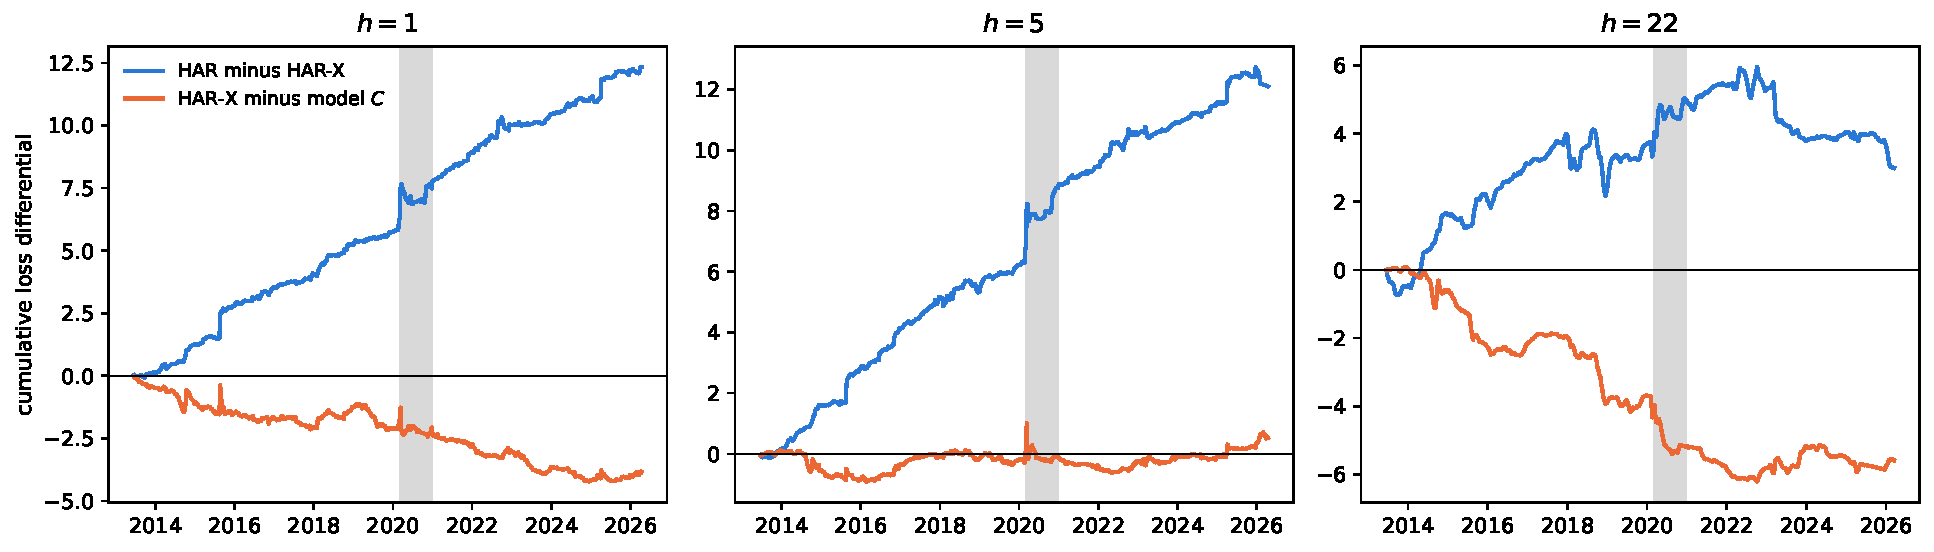
\includegraphics[width=\textwidth]{figures/fig_cumulative.pdf}
\caption{Cumulative sum over forecast origins of the cross-sectional mean
squared-error differential. Blue: HAR minus HAR-X (rising when implied
volatility helps). Orange: HAR-X minus model $C$ (rising when persistence
helps beyond implied volatility). Common cells; shading marks March to
December 2020.}
\label{fig:cumulative}
\end{figure}

\subsection{Information timing}

The comparison between HAR and HAR-X is sensitive to a detail that is easy
to get wrong. If the HAR terms are built from variance through day $t-1$,
for example by lagging the regressors one day to avoid look-ahead, while the
VIX is the close of day $t$, the implied-volatility model receives one more
day of information than the benchmark. Table~\ref{tab:timing} re-estimates
both models with HAR inputs ending at $t-1$ and compares them with the
aligned versions used elsewhere in the paper.

\begin{table}[H]
\caption{Information timing and the apparent value of implied volatility.}
\label{tab:timing}
\small
\begin{tabularx}{\textwidth}{Xcrrr}
\toprule
HAR inputs & $h$ & MSE HAR & MSE HAR-X & HAR-X gain (DM) \\
\midrule
Through $t-1$ & 1 & 0.6691 & 0.6350 & +5.11\% (+4.56) \\
 & 5 & 0.3637 & 0.3354 & +7.76\% (+4.62) \\
 & 22 & 0.2712 & 0.2633 & +2.90\% (+1.46) \\
\midrule
Through $t$ & 1 & 0.6146 & 0.5955 & +3.11\% (+5.23) \\
 & 5 & 0.3381 & 0.3193 & +5.54\% (+5.35) \\
 & 22 & 0.2632 & 0.2586 & +1.77\% (+0.95) \\
\midrule
HAR, $t$ vs $t-1$ & 1 & & & +8.15\% (+6.39) \\
 & 5 & & & +7.04\% (+5.00) \\
 & 22 & & & +2.93\% (+3.41) \\
\bottomrule
\end{tabularx}
\noindent{\footnotesize{\textit{Notes:} VIX and MOVE are closes of the origin day $t$ in every row. Through $t-1$: HAR terms built from variance through the day before the origin and the previous day's return. Through $t$: the aligned specification used everywhere else. Common cells of all four forecast panels; DM statistics in parentheses.}}
\end{table}


Aligning the inputs lowers HAR's error by 8.1\% at one day, 7.0\% at one week
and 2.9\% at one month, all significant. Because HAR-X already contains the
day-$t$ VIX, it gains less from the alignment, and its advantage over HAR
falls from 5.1\% to 3.1\%, from 7.8\% to 5.5\% and from 2.9\% to 1.8\%. Between
29\% and 39\% of the apparent value of implied volatility is a timing
artefact. Earlier versions of this study used the misaligned convention and
reported the larger gains; any study that compares HAR with implied-volatility
regressors should check the same alignment.

\subsection{Three designs that give persistence a better chance}

Three objections to the per-stock design are natural, and Table~\ref{tab:designs}
answers each with a design registered before its results were computed.

\begin{table}[H]
\caption{Three designs that give persistence a better chance.}
\label{tab:designs}
\footnotesize
\begin{tabularx}{\textwidth}{lXcrrr}
\toprule
Design & Comparison & $h$ & $\Delta$MSE & DM & CW $p$ (Holm) \\
\midrule
Pooled, fixed effects & Full model vs HAR-X & 1 & +0.40\% & +1.19 & 0.000 \\
 &  & 5 & +0.34\% & +0.79 & 0.000 \\
 &  & 22 & -1.36\% & -1.30 & 0.627 \\
 & HAR-X + cross-sectional state vs HAR-X & 1 & +0.34\% & +1.18 & 0.004 \\
 &  & 5 & +0.19\% & +0.53 & 0.016 \\
 &  & 22 & -1.00\% & -0.96 & 0.627 \\
\midrule
Duration target & Full model vs HAR-X & 22 & -1.81\% & -3.92$^{***}$ & 0.026 \\
 & HAR-X + cross-sectional state vs HAR-X & 22 & -0.35\% & -1.42 & 0.677 \\
\midrule
Market level & Full market model vs market HAR-X & 1 & +3.42\% & +1.77$^{*}$ & 0.000 \\
 &  & 5 & +2.01\% & +1.45 & 0.000 \\
 &  & 22 & -1.93\% & -1.00 & 0.270 \\
\bottomrule
\end{tabularx}
\noindent{\footnotesize{\textit{Notes:} Pooled: one regression across stocks with stock fixed effects (within transformation on training means), refit at every origin. Duration target: log ratio of mean future variance over 22 and 5 days. Market level: one series, the cross-sectional mean of the stock targets, with market HAR terms, VIX, MOVE and the persistence state. Each design was specified before its results were seen.}}
\end{table}


First, per-stock regressions estimate many coefficients from about 650 weekly
observations, and the persistence state is common to all stocks. A pooled
regression with stock fixed effects estimates each coefficient once from the
whole panel. Pooling helps: model $C$ now beats pooled HAR-X by 0.40\% at one
day and 0.34\% at one week, and the Clark--West rejections survive Holm
adjustment. But the gains are well below the 0.5\% threshold and not
significant by Diebold--Mariano, and at one month the sign reverses.

Second, persistence might describe how long volatility stays high rather
than how high it is. We therefore forecast the slope of the variance term
structure, the log ratio of mean variance over the next 22 days to mean
variance over the next 5. HAR beats an expanding-mean benchmark on this target
by 3.3\%, so the slope is forecastable, but adding persistence to HAR-X makes the
forecasts worse, significantly so for model $C$ ($-1.8\%$, $t=-3.92$).

Third, the state is a market-wide quantity and may be visible only at the
market level. On a single series, the cross-sectional mean of the stock
targets, the persistence state improves on a market HAR-X by 3.4\% at one day
and 2.0\% at one week, with Diebold--Mariano statistics of 1.77 and 1.45. This
is the largest gain in the study, but with one series and 646 origins it is
not significant, and Appendix~\ref{app:market} shows that it is carried by a
known quantity: the trailing gap between implied and realized variance,
which captures the variance risk premium, absorbs it.

\subsection{Calm and stressed periods}

Splitting the evaluation period by the quartiles of the VIX on the forecast
dates gives no sign of a regime in which persistence pays. In the highest
VIX quartile model $C$ improves on HAR-X by 2.4 percentage points at one week,
with a Diebold--Mariano statistic of 1.36; in the lowest quartile it is
worse at every horizon; during March to December 2020 it is 0.2 points
worse at one week and 5.6 points worse at one month. With 162 dates per
quartile and 43 in 2020 these comparisons are descriptive.

\section{Robustness and Economic Value}\label{sec:robust}

\subsection{Estimators, windows, targets and learners}

Panel A of Table~\ref{tab:robust} varies the construction of the persistence
predictors and the target at the weekly horizon, where model $C$ performs
best. Its gain over HAR remains between 5.2\% and 6.4\% when $d$ is estimated
by local Whittle instead of GPH, over 500 or 1000 days instead of 750, or for
the more or less liquid half of the sample, and it is 2.6\% when the target
is the mean squared return. Each gain is of the same order as that of HAR-X
in the baseline, so none of these choices alters the conclusions of
Section~\ref{sec:results}. A GARCH(1,1) forecast, corrected point-in-time for
its level, is 19.9\% worse than HAR, consistent with the HAR family being the
stronger benchmark for range-based variance.

\begin{table}[H]
\caption{Robustness of model $C$ at $h=5$, and the machine-learning estimators.}
\label{tab:robust}
\footnotesize
\begin{tabularx}{\textwidth}{Xrr}
\toprule
\multicolumn{3}{l}{\textit{Panel A. Model $C$ versus HAR at $h=5$}} \\
\midrule
Variant & $\Delta$MSE vs HAR & DM \\
\midrule
Headline (GPH, $W=750$) & +5.79\% & +4.22$^{***}$ \\
Local Whittle instead of GPH & +5.98\% & +4.13$^{***}$ \\
Window 500 days & +5.33\% & +3.56$^{***}$ \\
Window 1000 days & +6.19\% & +4.16$^{***}$ \\
Target: squared returns & +2.63\% & +2.89$^{***}$ \\
Less liquid half & +6.36\% & +4.16$^{***}$ \\
More liquid half & +5.19\% & +3.98$^{***}$ \\
GARCH(1,1) instead of model $C$ & -19.94\% & -9.04$^{***}$ \\
\midrule
\multicolumn{3}{l}{\textit{Panel B. Model $D$: model $C$'s predictors, other estimators ($\Delta$MSE vs HAR-X at $h=1$ / $5$ / $22$)}} \\
\midrule
Estimator & $\Delta$MSE & DM \\
\midrule
Lasso & -0.8\% / -1.3\% / -3.1\% & -2.6 / -2.2 / -2.6 \\
Ridge & -1.5\% / -1.9\% / -4.2\% & -3.7 / -2.6 / -3.0 \\
Elastic net & -0.8\% / -1.4\% / -3.3\% & -2.5 / -2.2 / -2.5 \\
Random forest & -5.8\% / -6.2\% / -7.0\% & -4.5 / -3.9 / -3.2 \\
Gradient boosting & -6.2\% / -6.1\% / -10.3\% & -6.2 / -5.4 / -4.2 \\
\bottomrule
\end{tabularx}
\noindent{\footnotesize{\textit{Notes:} Panel A: percentage MSE reduction of model $C$ relative to HAR at $h=5$ under each variant; the GARCH row compares a level-corrected GARCH(1,1) forecast with HAR. Panel B: shrinkage hyperparameters and gradient-boosting tree size, leaf size and number of trees chosen by time-series cross-validation inside each training window; the random forest uses 200 trees with a minimum leaf of 20; refit every 20 weeks.}}
\end{table}


Panel B replaces the linear regression on the 18 predictors of model $C$ by
five machine-learning estimators: the lasso, ridge regression and the elastic
net, whose penalties are chosen by time-series cross-validation within each
training window; a random forest; and gradient boosting, whose tree size,
minimum leaf size and number of trees are chosen in the same way. All five
are significantly worse than HAR-X at every horizon. The shrinkage
estimators lose 0.8\% to 4.2\%, and the tree ensembles 5.8\% to 10.3\%. In
this sample, neither regularization nor nonlinearity extracts information
from the persistence predictors that the linear HAR-X model misses. Tuning
matters for this conclusion: gradient boosting with fixed default settings
(400 trees with 31 leaves) loses 12\% to 21\% relative to HAR, an artifact of
overfitting 430 to about 1070 training observations that tuning largely
removes.

\subsection{Volatility-managed portfolios}

A forecast that is statistically no more accurate can still be economically
useful. We examine this with the volatility management of
\citet{moreira2017volatility}, applied stock by stock: each week the
position in stock $i$ is scaled by $c_{i,t}/\hat\sigma^2_{i,t+5\mid t}$,
where $\hat\sigma^2_{i,t+5\mid t}$ is the weekly-horizon variance forecast of
a given model and $c_{i,t}$ is set in real time so that the managed and
unmanaged positions have the same past variance. Positions are funded at the
three-month Treasury bill rate, and returns are measured in excess of it. In
addition to the HAR, HAR-X and model $C$ forecasts, we include a model-free
rule that scales positions by trailing 22-day variance.

\begin{table}[H]
\caption{Volatility-managed portfolios (excess returns, weekly, 2014--2026).}
\label{tab:portfolios}
\footnotesize
\begin{tabularx}{\textwidth}{Xrrrrr}
\toprule
Portfolio & Sharpe & Sharpe, 10 bp & Turnover & Sharpe, COVID & Max drawdown \\
\midrule
Equal weight & 0.76 & 0.76 & 1.1 & 0.88 & -30.6\% \\
Trailing 22-day variance & 0.76 & 0.69 & 6.6 & 1.09 & -15.7\% \\
HAR & 0.75 & 0.64 & 11.5 & 1.29 & -17.3\% \\
HAR-X & 0.76 & 0.66 & 10.5 & 1.38 & -15.6\% \\
Model $C$ & 0.76 & 0.66 & 10.3 & 1.62 & -15.8\% \\
\bottomrule
\end{tabularx}
\noindent{\footnotesize{\textit{Notes:} Each stock's position is scaled by $c_{i,t}/\hat\sigma^2_{i,t+5|t}$ with $c_{i,t}$ set in real time so that the managed and unmanaged positions have equal past variance; positions are funded at the three-month Treasury bill rate; 594 weeks after a 52-week warm-up. Turnover: notional traded per unit of capital per year, including drift. COVID: March to December 2020 (43 weeks). Sharpe differences, Ledoit--Wolf HAC $p$ (block bootstrap $p$): model $C$ vs HAR-X 0.94 (0.93) full sample, 0.10 (0.31) COVID; model $C$ vs equal weight 0.97 (0.98).}}
\end{table}


Table~\ref{tab:portfolios} shows no economic value from any of the forecasts.
Every managed portfolio has a full-sample Sharpe ratio of 0.75 or 0.76, equal
to that of the equal-weighted portfolio, and none of the differences is close
to significant. Management lowers volatility and roughly halves the maximum
drawdown, but it reduces expected excess returns in proportion. The managed
portfolios trade about ten times their capital each year, and at a cost of
10 basis points per unit traded their Sharpe ratios fall to 0.64--0.66, below
that of equal weighting. The one period in which model $C$ stands out, March
to December 2020, contains 43 weekly observations, and its advantage over
HAR-X in that period (a Sharpe ratio of 1.62 against 1.38) is not
significant. These results are in line with the evidence that volatility
management of factor portfolios is fragile out of sample
\citep{cederburg2020volatility, barroso2021volatility}.

\section{Discussion}\label{sec:discussion}

\subsection{Why persistence does not improve forecasts}

Section~\ref{sec:window} shows that the rolling persistence state is largely
a smoothed record of the largest volatility episodes of the preceding two to
four years. It rises when such an episode enters the window and falls, on a
date fixed by the window length, when the episode leaves.
Sections~\ref{sec:results} and \ref{sec:robust} show that, once the VIX and
MOVE are in the model, the state does not significantly improve forecasts in
any of the registered designs. We interpret the first result as the
explanation for the second. Implied volatility is a forward-looking price
that already reflects recent turmoil, partly through a variance risk premium
that rises after crises and decays slowly \citep{bates2000post,
bekaert2014vix, andersen2015risk}. A backward-looking indicator of when the
last crisis occurred has little to add. The Clark--West rejections show that
it adds some information in population; the Giacomini--White tests show that
this contribution is too small to survive estimation.

These results do not imply that volatility lacks long memory, or that the
persistence of volatility shocks never changes. The full-sample estimates in
Table~\ref{tab:memory} are large, and our short-memory null reproduces their
calm-period level, consistent with a long literature showing that level
shifts and long memory are difficult to separate \citep{diebold2001long,
perron2010long, varneskov2018combining}. Our claim is narrower: the time
variation in rolling estimates is not evidence of time variation in
persistence. It is the pattern that a process with constant parameters
produces when a few large episodes pass through a fixed window.

\subsection{Implications for applied work}

Three practices follow for research that uses rolling memory estimates,
Hurst exponents or similar windowed statistics. First, results should be
reported for several window lengths, with a check of whether the turning
points move with the window; a structural change should not. Second, the
windowed statistic can be regressed on the largest value of an observable
stress measure inside the same window; a high $R^2$ indicates that the
statistic reflects window composition rather than dynamics. Third, the
series can be compared with a short-memory null into which the observed
episodes are injected, and with estimators and tests designed to separate
long memory from level shifts \citep{qu2011test, hou2014modified}. These are
standard tools in fields that encountered the same problem earlier, from
hydrology \citep{klemes1974hurst} to early-warning indicators in ecology and
climate science \citep{dakos2008slowing, ditlevsen2010tipping,
boettiger2012quantifying} and sliding-window connectivity in neuroscience
\citep{leonardi2015spurious}.

Three lessons for forecasting studies extend beyond this application. The
benchmark and the challenger must use the same information set, down to the
day: a one-day lag in the inputs of the benchmark inflated the value of
implied volatility by about a third. When a nested comparison yields a
Clark--West rejection without a lower loss, a Giacomini--White test indicates
whether the estimated model is useful. Finally, machine-learning comparisons
are informative only if every learner is tuned under the same protocol: with
default settings gradient boosting lost 12--21\% relative to HAR, against
0.2--8\% once tuned.

\subsection{Limitations}

The panel consists of current S\&P~500 members with long histories. Firms
that left the index are missing, which removes some of the most volatile
histories; this omission affects the level of volatility and of the memory
estimates more than the window mechanism, which is a property of the
estimator. The variance proxy is the daily range rather than intraday
realized variance. Its sampling noise lowers the level of $\hat d$ and of the
Hurst exponent but does not change the dates at which episodes enter and
leave the window. Returns are price returns, which matters only for the
portfolio exercise. The forecast evaluation period, 2013 to 2026, contains
one extreme episode, in 2020, and several moderate ones; the window analysis
also uses 2008. Markets without a liquid implied-volatility index are where
persistence could add the most, but in such markets the largest recent
realized variance is directly available and would be the natural benchmark.
Finally, the evidence on the window mechanism concerns memory in volatility;
a general analysis across estimators, asset classes and markets is left for
future work.

\section{Conclusions}\label{sec:conclusions}

Rolling long-memory estimates of stock volatility rise sharply in crises, and
it is tempting to read them as a measure of how persistent the market has
become. For 115 S\&P~500 stocks over 2001--2026 they do not improve
volatility forecasts beyond implied volatility under any design we
registered: per-stock and pooled regressions, the level and the term
structure of future variance, a market-level series, linear models and tuned
machine-learning estimators, calm and stressed periods, and
volatility-managed portfolios. The evidence points to a simple reason: the
rolling persistence state records which extreme episodes lie inside its
window. It jumps when an episode enters and falls when the episode leaves, at
dates that move one-for-one with the window length; a short-memory process
reproduces this pattern; and 83\% of its variation is explained by the
largest VIX inside the window. Researchers who use rolling memory estimates
as a state variable should check for these signatures before interpreting
them. Forecasting studies that compare HAR with implied volatility should
align the information sets of the two models, which here removes a third of
the apparent value of the VIX.


\vspace{6pt}

\authorcontributions{CO-AUTHORS TO CONFIRM. Conceptualization, A.D., N.A.,
H.M. and S.T.R.; methodology, A.D. and H.M.; software, A.D.; formal analysis,
A.D.; data curation, N.A.; writing---original draft preparation, A.D.;
writing---review and editing, A.D., N.A., H.M. and S.T.R.; supervision,
S.T.R.}

\funding{This research received no external funding.}

\institutionalreview{Not applicable.}

\informedconsent{Not applicable.}

\dataavailability{Daily prices, ranges and index levels were obtained from
Bloomberg and cannot be redistributed. The full code, the experiment ledger
with every specification and its date of registration, and the derived
results are available at \url{https://github.com/akashdeepo/LRD-ML}.}

\acknowledgments{CO-AUTHORS TO CONFIRM the generative-AI statement required by
MDPI: state which tools were used, for which tasks (for example code review,
analysis scripts, drafting and editing), and that the authors reviewed and take
responsibility for the content.}

\conflictsofinterest{The authors declare no conflicts of interest.}

\appendixtitles{yes}
\appendixstart
\appendix
\section[\appendixname~\thesection]{Roughness at the daily frequency}\label{app:rough}

The increment-scaling estimate of the Hurst exponent of daily log Parkinson
variance averages 0.060 across stocks (10th--90th percentile 0.053--0.069).
Read literally, this indicates volatility much rougher than Brownian motion,
for which the exponent is 0.5. We ask whether a
process without fractional roughness, observed through the Parkinson
estimator, produces the same value. Latent log variance is the sum of two
independent AR(1) components, a Markovian model. The observed series adds the
sampling error of the range estimator, $\eta_t = \ln(R_t^2/4\ln 2)$ minus its
mean, where $R_t$ is the range of a standard Brownian motion over one day
sampled at 390 one-minute steps; its variance, 0.36, is fixed by theory and
is about a third of the variance of observed log variance. The two
autoregressive coefficients and the variance split are fitted to the median
autocorrelations of observed log variance at nine lags from 1 to 250 days,
which gives a fast component with coefficient 0.66 and a slow one with
coefficient 0.995. Over 200 simulated paths of 6136 days the same estimator
gives 0.064 (standard deviation 0.004) on the observed series, matching the
data, and 0.19 on the noise-free latent series. Two features of daily data
therefore produce the low estimate without any roughness: the sampling noise
of the range, which lowers the estimate from 0.19 to 0.06, and a fast
mean-reverting component, which already holds it well below 0.5 at lags of up
to 21 days. Daily range data cannot identify roughness, in line with
\citet{cont2024rough}. The code is module 16 of the repository.

\section[\appendixname~\thesection]{Additional forecast results}\label{app:extra}

\textit{QLIKE.} Variance forecasts are obtained from the log forecasts with a
point-in-time smearing correction: the mean of the exponentiated past
out-of-sample errors whose targets had been observed by the origin, with at
least 26 such errors. Against HAR-X, no specification has a significantly
lower QLIKE loss at the 5\% level; the largest Diebold--Mariano statistic in
favor of persistence is 1.67 (cross-sectional extension, one day), and model
$C$ is significantly worse at one month ($-2.08$).

\textit{Machine learning.} The lasso, ridge and elastic-net penalties are
chosen by five-fold expanding time-series cross-validation with a gap of
$\lceil h/5\rceil$ rows between training and validation folds. Gradient
boosting (LightGBM, learning rate 0.05) chooses the number of leaves
$\{2,4,15\}$, the minimum leaf size $\{20,50\}$ and the number of trees
$\{25,\dots,800\}$ by three-fold time-series cross-validation in each
training window. The random forest uses 200 trees with a minimum leaf of 20.
Each learner is refit every 20 weeks on the embargoed training rows. With
fixed defaults (400 trees, 31 leaves) gradient boosting loses 15.9\%,
11.9\% and 21.2\% to HAR at the three horizons; tuned, it loses 2.9\%, 0.2\%
and 8.3\%.

\section[\appendixname~\thesection]{The market-level gain}\label{app:market}

On the market-level series the persistence state improves on market HAR-X by
3.4\% and 2.0\% at one day and one week (Table~\ref{tab:designs}). An
exploratory analysis, specified after that result and therefore not a formal
test, asks what accounts for the gain. In a specification in levels, the
interaction of the VIX with the logarithm of its maximum over the previous
three years has a negative coefficient ($t=-2.7$ at both horizons): the
slope of future realized variance on the VIX is about 40\% lower when a
crisis is recent. In logs the interaction disappears ($t=0.33$ and $0.26$),
and the three-year maximum enters only as a level shift, which is absorbed
by the trailing 250-day gap between VIX-implied and realized variance. That
gap alone improves on the log market HAR-X model by 5.0\% to 6.3\%
(Diebold--Mariano statistics of 2.7 to 3.5). The market-level gain is
therefore best interpreted as the slowly decaying variance risk premium after
crises \citep{bates2000post, andersen2015risk}, for which the persistence
state may act as a proxy because both depend on how recently the last crisis
occurred. A test of this interpretation requires data not used here, such as
earlier index history or other markets.

\section[\appendixname~\thesection]{Registration record and audit}\label{app:ledger}

The study was carried out in stages. Before each stage the specifications,
comparisons, tests and decision rules were written into an experiment ledger
kept under version control; results were added afterwards and earlier entries
were not edited. The ledger, the code and a list of every correction are in
the repository named in the Data Availability Statement. The main stages
were:
\begin{itemize}
\item an embargo on training observations whose targets were not yet
realized at the origin, which removed an apparent gain of the persistence
model at the monthly horizon;
\item three HAR-X extensions with a fixed decision rule and Holm adjustment;
\item pooled, term-structure and market-level designs, point-in-time
winsorization and real-time portfolio normalization;
\item a full audit of the pipeline, whose corrections were registered before
the final run: aligned information timing (Table~\ref{tab:timing}), missing
rather than floored zero-range days, memory estimated on log variance
throughout, a Newey--West bandwidth that grows with the sample, point-in-time
QLIKE, time-series cross-validation for every learner, a level-corrected
GARCH benchmark, common evaluation cells and dates, and portfolio returns in
excess of the bill rate;
\item the window-inclusion analysis (Table~\ref{tab:window}), the
Giacomini--White tests and the timing comparison, each registered with a
prediction before it was run.
\end{itemize}
% CO-AUTHORS: decide whether to add one sentence noting that an earlier
% version (arXiv:2605.24285) reported larger gains, and that the
% differences come from the corrections listed above.


\begin{adjustwidth}{-\extralength}{0cm}
\reftitle{References}
\bibliography{references}
\end{adjustwidth}

\end{document}
